\documentclass[12pt,letterpaper]{article}

%==================================================================================
% Template for the 13th International Association of Fire Safety Science (2019).  
%==================================================================================

% This template is based on the layout requirements of the Fire Safety Journal.  When submitting, please do include the *.tex and output (typeset) *.pdf files, figure files (photographs, diagrams, etc.), and any other ancillary files required to typeset your article.  The journal must be able to typeset your article with what you've provided.

% As with any programming language, there are multiple ways of executing any given task (e.g., figures, tables, maths, etc.).  The syntax in this template should be considered suggestions and not directives.  Please feel free to use your own favorite syntax, especially if it's more elegant than what is found below!  That said, the spacing and font parameters have been selected to conform to the appearance dictated by the journal (i.e. like MS Word).  Make sure your final typeset document has the correct formatting or it will be rejected.

% Required Packages ===============================================================
\usepackage{amsmath} % The usual maths package
\usepackage{amsfonts}  % The usual maths package
\usepackage{amssymb}  % The usual maths package
\usepackage[final]{graphicx} %Required for figures.
\usepackage{caption} % Needed to modify default figure captions
\usepackage{latexsym}
\usepackage{lineno} % Enables line numbers
\usepackage{parskip} % Makes a space between paragraphs like MS word
\usepackage{fullpage} % Overrides article margins
\usepackage{titlesec} % Enables modification of section labels
\usepackage[numbib]{tocbibind} %Make References a numbered section
\usepackage{siunitx} % Formats the units and values
\usepackage{times}
\usepackage{chemformula}


%\usepackage{subcaption} % Enables multiple images in one figure environment
%\usepackage{xcolor} % For various font colors in figures
%===================================================================================

% The next two lines modify the font and font size of the section and subsection labels
\titleformat{\section}{\normalfont\bfseries}{\thesection}{0.2em.}{}
\titleformat{\subsection}{\normalfont\bfseries}{\thesubsection}{0.2em}{}

% This will change the figure captions from the default "Figure 1:" to "Fig. 1."
\captionsetup[figure]{labelformat={default},labelsep=period,name={Fig.}}

\linenumbers % Include line numbers throughout document

\begin{document} %====================================================================
\begin{flushleft} % Suppress the default full justification of text

% Title of your article
\textbf{Backdraft: Exeriments and Large Eddy Simulations in a scaled compartment}
\vspace{3mm}\\
%
% Author(s)
Marcos Vanella$^\text{a*}$, Ryan Falkenstein-Smith$^\text{a}$, and Thomas Cleary$^\text{a}$
\vspace{3mm}\\	

% Affiliation "b"
$^\text{a}$National Institute of Standards and Technology, 100 Bureau Drive, MS 8661, Gaithersburg, USA  \\
marcos.vanella@nist.gov
\vspace{3mm}

$^*$Corresponding author

% Highlights/keywords ===================================================
\textbf{Highlights:}	
\begin{itemize}
	\itemsep-4pt % Override default vertical spacing among list items
	\item Three to five bullet points
	\item Each to have a maximum of 85 characters, including spaces
	\item Cover main findings
	\item Usually submitted separately
\end{itemize}
\vspace{3mm}

% Abstract ==============================================================	
\textbf{Abstract:}
\vspace{3mm}
An extensive set of backdraft experiments has been performed at the NIST National Fire Research Laboratory. These experiments were conducted in a 2/5 scale ASTM standard compartment and are part of an effort the define the conditions at which backdraft can arise. Also, the detailed chemistry and heat measurements are intended to evaluate computer code fire models. In this article we describe the modeling effort employing the Fire Dynamics Simulator (FDS) in a set of simulations involving different fuels and ingnition source locations mirroring a subset of the named experiments. We focus in the use of default simulation parameters and their effect on the backdraft outcomes. In particular it is noted that the temperature threshold of the ignition model plays a primary role in the development of backdraft.

\textbf{Keywords:}

Backdraft; Fire Simulation; FDS; Large Eddy Simulation; 

\section{Introduction}
Backdrafts pose a life-threatening risk to any firefighter that may encounter them. A backdraft is a deflagration resulting from igniting an incoming gravity current of air mixed with a heated, fuel-rich, and oxygen-depleted environment~\cite{fleischmann2013defining}. Several experimental works have identified the physical mechanisms and conditions conducive to backdrafts. Fleischmann examined the thermal and gas compositions within an enclosure's environment influencing the incoming gravity current~\cite{fleischmann1993backdraft,fleischmann1994quantitative}. Gottuk and others estimated critical mass fractions in vitiated atmospheres that result in backdraft on a full scale using steel compartments. Wu et al. established a correlation between the likelihood of backdraft and compartment configuration by varying ventilation conditions, ignition locations, and mass fluxes of gas leakage~\cite{wu2011experimental}. Other works have studied the probability of backdraft generated from solid fuel combustion within an enclosure~\cite{hayasaka2008backdraft,tsai2013full,zhao2021experimental}.

%\textbf{Falkenstein-Smith R. and Cleary Thomas (2022):} Over 500 tests varying the type of fuel, fuel load, door window geometry, spark location in compartment. Temperature, species composition, in several probes within the compartment, heat flux probes in-outside of compartment, HRR from oxygen consumption calorimetry.

%Falkenstein-Smith R. and Cleary Thomas, “Thermal and gas mixture composition preceding backdrafts in a 2/5th scale compartment,” NIST Technical Note, September 2022

Other works have relied on computational models to study backdraft. \textbf{Marcos: FDS simulation of Backdraft in the literature}

\textbf{Weng, Fan and Hasemi* (2005):}
Comparatively use simulations to study compartment geometry/bcs in gravity current to predict time of ignition of backdraft.


\textbf{Ferraris and others X (2008):}
Used a subgrid scale model based on mixture fraction progress variable to define partially premixed combustion applied to backdraft. Qualitative results.


\textbf{Park and others O (2017):} Park, Bo Oh, Shik Han, Hyung Do: Effects of initial fuel mass in backdraft, finite chemistry (one and three step reaction).


\textbf{Myilsamy and others + (2019):} Myilsamy and others: Mixing controlled fast chemistry. Studied effect of opening geometry in the critical fuel fraction was studied.


\textbf{Ashok and Echekki # (2021):} Ashok and Echekki: study the effect of gravity magnitude on backdraft events. 

*Weng W.G. et al., “Prediction of the formation of backdraft in a compartment based on large eddy simulation,” Engineering Computations, Vol. 22 No. 4, pp. 376-392 (2005).

X Ferraris S.A. et al., “Large eddy simulation of the backdraft phenomenon,” Fire Safety Journal 43:3, pp. 205-225 (2008).

O Park J.W. et. Al, “Computational study of backdraft dynamics and the effects of initial conditions in the compartment,” J. Mech. Sci. and Tech. 31:2, pp. 985-993 (2017).

+ Myilsamy D. et al., “Large eddy simulation of the backdraft dynamics in compartments with different opening geometries,” J. Mech. Sci. and Tech. 33:5, pp. 2189-2201 (2019).

# Ashok S.G. and Echekki T., “A numerical study of backdraft phenomena under normal and reduced gravity,” Fire Safety Journal 121 103270 (2021).


\textbf{What are we trying to do here?} Leverage the wealth of experimental data produced to assess the FDS default LES combusiton models in this challenging problem.  EDC -> Extra Extinction and re-ignition models arise their issues and advantages. 

Recently, an extensive series of 500 experiments, focused on examining backdraft in a reduced-scale enclosure, was performed at the NIST National Fire Research Laboratory~\cite{Falkenstein2022}. The experimental series generated a significant dataset that identifies environmental conditions indicative of backdraft.  

\textbf{Short description of the sections of the paper.}

\section{Experimental Method: Definition of compartment initial conditions}
A schematic of the 1~m~by~1~m~by~1.5~m reduced-scale enclosure used for all experiments is provided in Fig.~\ref{fig:Backdraft_experimental_setup}. The enclosure was designed to scale, 2/5\textsuperscript{th} the dimensions of an ASTM test room. Experiments were initiated when a square sand burner, with a 17.8~cm side length, was ignited. In these experiments, the sand burner's center was approximately 0.5~m from either side wall and 1.25~m from the front opening. After the initial ignition, the fire size increased to a predetermined heat release rate and was allowed to burn with the compartment door open for 60.0~s. Afterward, the door was shut. While the doorway was closed, fuel continued to flow through the burner for a predetermined duration, and when reached, the flow was zeroed. The fuel flow durations used in this work are shown in Table~\ref{tab:Fuel_Flow_Time}, corresponding to their respective fuel flow times. The compartment remained closed for an additional 30.0~s after the fuel flow duration to allow the internal gases to mix. Once the door opened, spark ignitors were prompted to arc, providing a potential ignition source for the residing fuel and incoming gravity current of air.
\begin{figure}[!]
	\centering
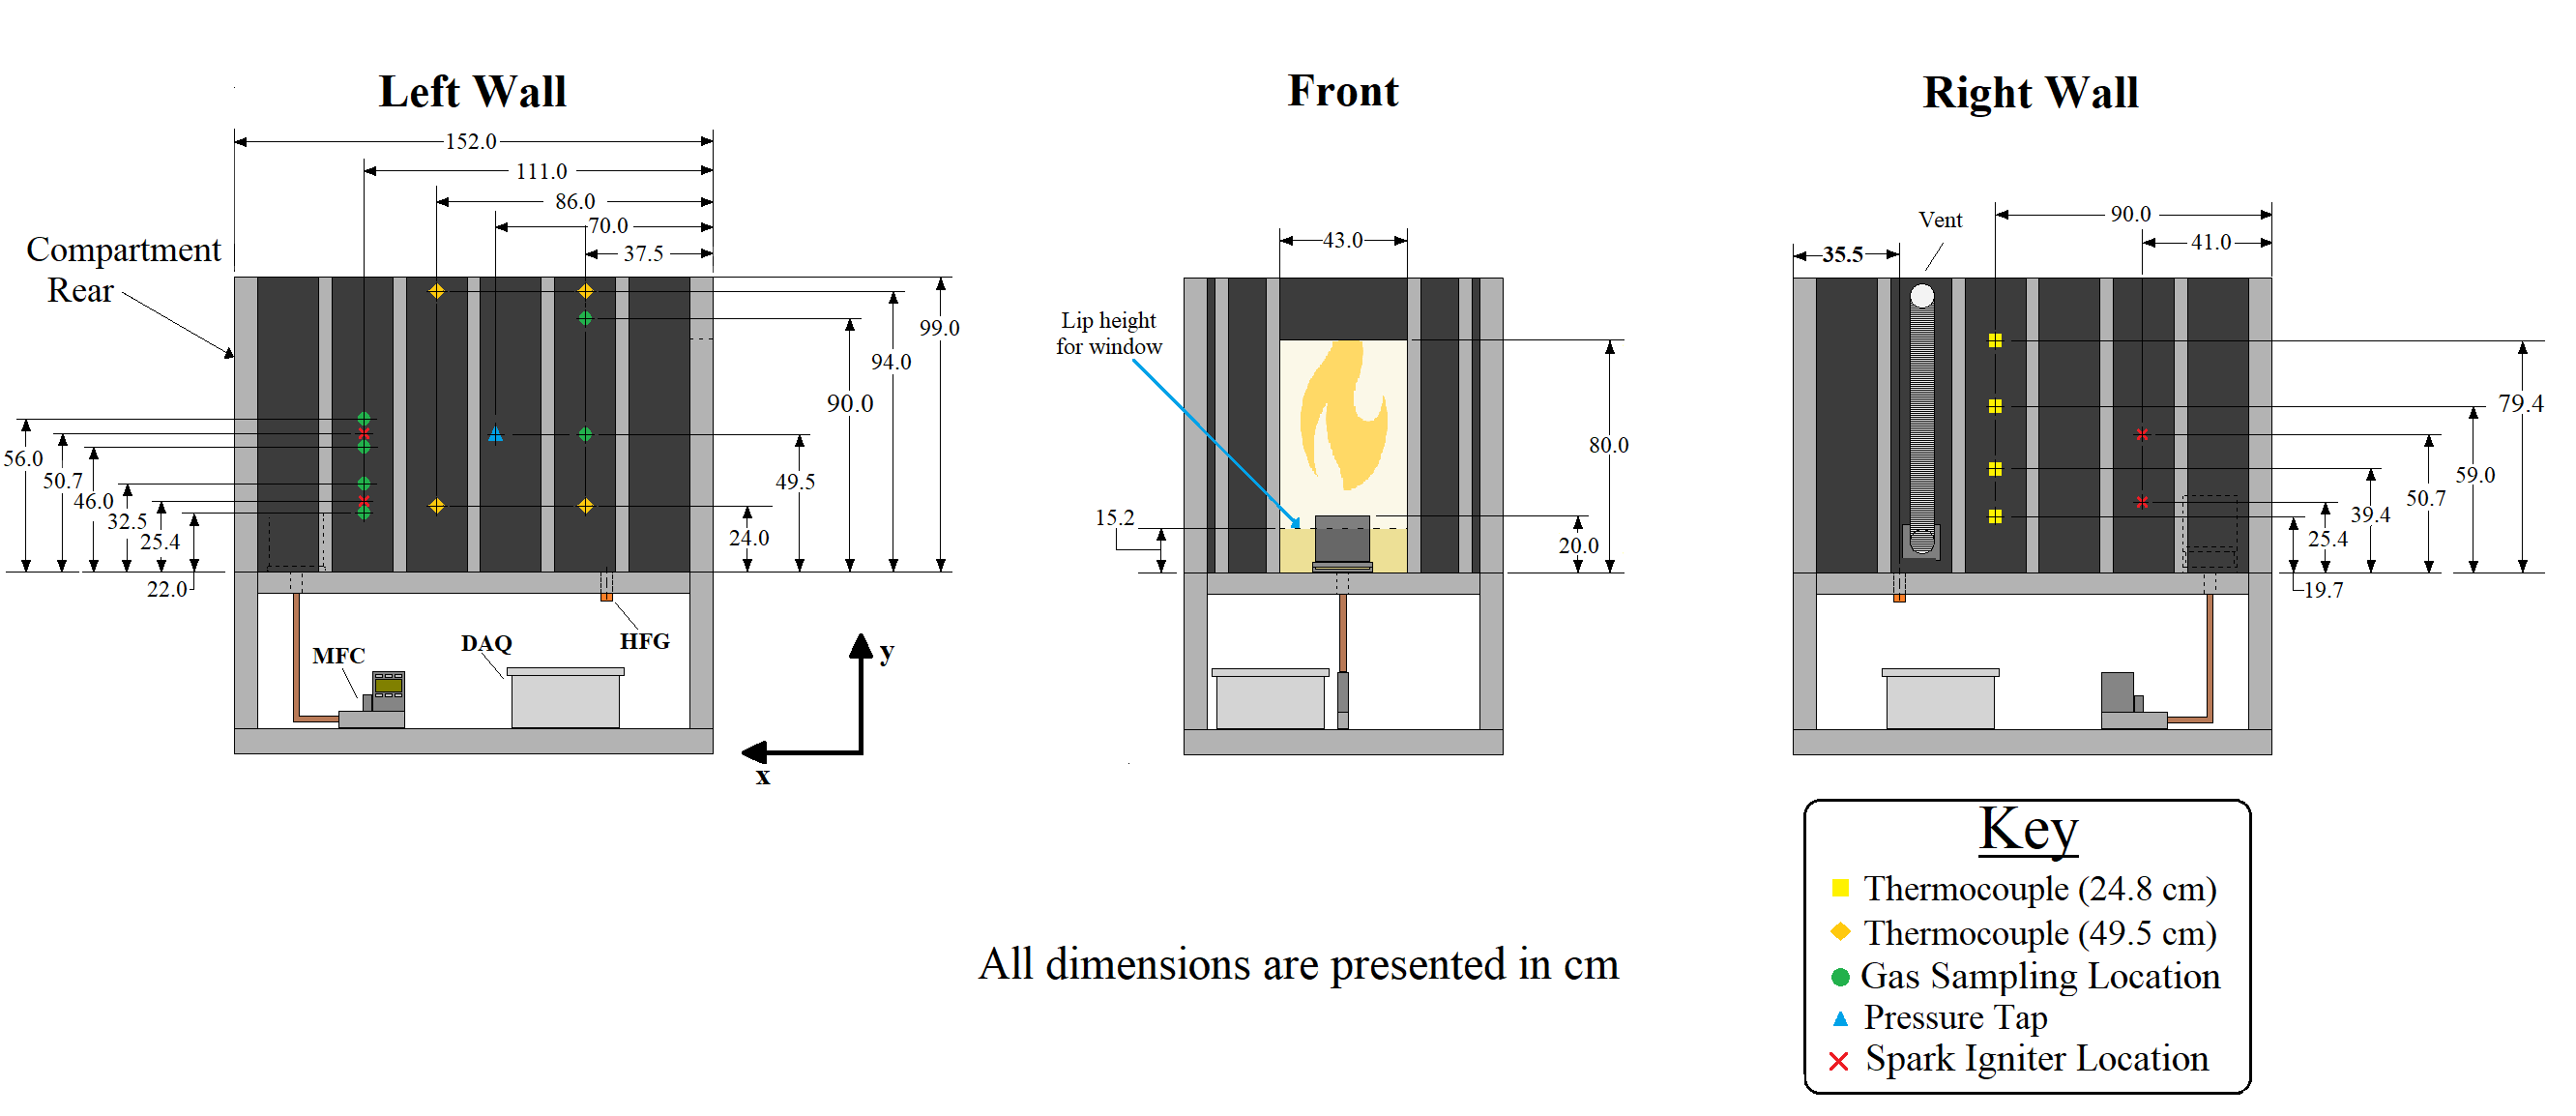
\includegraphics[width=16.0cm, keepaspectratio]{Experimental_Setup_6.png}
	\caption{Schematic of the $2/5^{\rm{th}}$ scale compartment used in backdraft experiments}
	\label{fig:Backdraft_experimental_setup}
\end{figure}

\begin{table}[h!]
\caption{List of fuel flow times for each fire configuration}
\label{tab:Fuel_Flow_Time}
\centering
	\footnotesize
	\begin{tabular}{c c l}
\hline
Fuel & Fire size~(kW)	& Fuel flow time~(s)  \\
\hline
Methane & 25.0~$\pm$~1.0~kW 	& 360,~390,~450\\
	& 37.5~$\pm$~1.0~kW 	& 225,~285      \\
%[0.075cm]
Propane & 16.7~$\pm$~1.0~kW		& 255,~270,~315	\\
	& 25.0~$\pm$~1.0~kW 	& 210,~285		 \\
\hline
\end{tabular}
\end{table}

The locations of the spark ignitors, thermocouples, and gas sampling locations are displayed in Fig.~\ref{fig:Backdraft_experimental_setup}. The spark ignitors were positioned either 25.4~cm ("low spark") or 50.7~cm ("mid spark") from the compartment floor. Thermocouples were incorporated on both side walls of the compartment in two different configurations. The first thermocouple configuration used 49.5 cm long, 0.3175 cm diameter sheathed Type K thermocouples configured in a rectangular orientation on the left wall facing the door. The second thermocouple array included four 24.8 cm long, 0.3175 cm diameter sheathed Type K thermocouples configured in a line on the right wall facing the door spaced approximately 19.9 cm apart. Gas samples were portioned and analyzed into two gas analyzers and phi meters at one of three location pairs displayed in Fig.~\ref{fig:Backdraft_experimental_setup}. The gas analyzer included one paramagnetic and two nondispersive infrared sensors to measure oxygen, carbon dioxide, and carbon monoxide. The phi meter~\cite{babrauskas1994phi,Falkenstein2021a} provided equivalence ratio measurements of the extracted gas sample. A combination of the gas analyzer and phi meter measurements was used to estimate the concentration of major species on a wet basis. Major gas species included methane/propane, oxygen, carbon dioxide, carbon monoxide, water vapor, and nitrogen. Gas and temperature measurements were monitored using a data acquisition system sampling 1.0~Hz during each experiment.

Initial conditions for backdraft models were determined in two-compartment zones from an averaged time-averaged temperature and estimated gas concentration measurements of repeated experiments with the same fuel flow duration and fire size. Zones were divided at the height of 40.0 cm from the species concentration measurements observed to be fairly homogeneous. Time-averaged measurements were calculated from a 10.0~s time domain immediately before the compartment doorway opening. The uncertainty of the initial conditions was determined from a combination of the Type A and B evaluation of uncertainty. The Type A evaluation of uncertainty was estimated from the variance of the averaged measurements. The Type B evaluation of uncertainty was determined from the reported instrumentation error. The variance between the averaged measurements was determined to be the dominant contributor to the estimated uncertainty.

Backdraft intensity was estimated from the total heat release of the exiting flame. During each experiment, the compartment was placed under a canopy hood with a 3.0~MW calorimetry measurement system. In this instance, the heat release rate was estimated using carbon dioxide generation calorimetry with a correction for carbon monoxide generation to account for unburned fuel exiting the compartment. The total heat release was calculated using Eq.~\ref{eq:total_heat_release_corr}:
\begin{equation}
\begin{split}
\label{eq:total_heat_release_corr}
THR&=\sum_{t=0}^{\infty} \left[ \dot{m}_{\rm{CO_2}}(t)\left(\frac{\rm{LHV_F}~\rm{MW_F}}{\rm{x}~\rm{MW_{CO_2}}}\right)+\dot{m}_{\rm{CO}}(t)\left(\frac{\rm{LHV_F}~\rm{MW_F}}{\rm{x}~\rm{MW_{CO}}}-\Delta\rm{H}^{\rm{o}}_{C,CO}\right) \right] \Delta~t
\end{split}
\end{equation}
Here, $\dot{m}_{\rm{CO_2}}(t)$ and $\dot{m}_{\rm{CO}}(t)$ represent the mass flow rate of \ch{CO2} and \ch{CO} measured in the duct, respectively. The number of carbon atoms and lower heating value of the parent fuel are represented by $\rm{x}$ and $\rm{LHV_F}$, respectively. The molecular weight of the parent fuel, carbon dioxide, and carbon monoxide is denoted as $\rm{MW_F}$, $\rm{MW_{CO_2}}$, and $\rm{MW_{CO}}$, respectively. The heat of combustion for carbon monoxide, $\Delta \rm{H}^{\rm{o}}_{C,CO}$ used in Eq.~\ref{eq:total_heat_release_corr} was 10.10~kJ/g as reported by Ref.~\cite{Hurley2016}. The heat released from the combustion gases trapped in the compartment before opening the door is subtracted from the measured total heat released for a backdraft.

\section{Numerical Method and Model setup}

\textbf{LES with Eddy dissipation concept, ignition and extinction, FDS numerics  LES vs VLES, model setup in Validation, chemistry, default parameters, geometry, grids.}



\section{Effect of Ignition Threshold}

\textbf{Re-ignition model:} History, options : Large value, AIT, tune it in this case. How do we do it?

\section{Backdraft simulation results}

\textbf{Backdraft probabilities, explanation, some physics results.}


\section{Conclusions}

\textbf{- Very challenging problem for fast chemistry calculations. - Ignition needs to be tuned. Comment on incorporating subgrid temperature fluctuations into the model. - Physics comparisons on selected cases, etc.}

\section*{References}
\bibliographystyle{elsarticle-num}
\bibliography{References}
	
%\begin{thebibliography}{9}
%	\bibitem{fleischmann2013defining}
%	C.M. Fleischmann and Z. Chen, 
%	``Defining the difference between backdraft and smoke explosions,'' 
%	Procedia Engineering,
%	vol. 62, pp. 324--330, 2013.
%	
%	\bibitem{guigay2009use}
%	G. Guigay, D. Gojkovic, L.G. Bengtsson, B. Karlsson, and J. Eliasson,
%	``The use of CFD calculations to evaluate fire-fighting tactics in a possible backdraft situation,''
%	Fire Technology,
%	vol. 45, no. 3, pp. 287--311, 2009.
%	
%	\bibitem{gojkovic2000initial}
%	D. Gojkovic
%	``Initial backdraft experiments,'' 
%	Technical Report 3121 
%	Lund University,
%	2000.
%
%	\bibitem{tsai2013full}
%	L.C. Tsai and C.W. Chiu,
%	``Full-scale experimental studies for backdraft using solid materials,''
%	Process Safety and Environmental Protection,
%	vol. 91, no. 3, pp. 202--212, 2013.	
%	
%	\bibitem{Parkes2009}
%	A.R. Parkes
%	''The Impact of Size and Location of Pool Fires on Compartment Fire Behaviour,''
	
	
	%\bibitem{quintiere_2017}
	%J. G. Quintiere, 
	%Principles of Fire Behavior, 
	%2nd edition, 
	%CRC Press, 
	%2017.
	
	%\bibitem{williams_1969}
	%F. Williams, 
	%``Scaling mass fires,'' 
	%in Fire Research Abstracts and Reviews, 
	%vol. 11, pp. 1-23, 1969.
		
	%\bibitem{emori_1982}
	%R. I. Emori and 
	%K. Saito, 
	%"Model experiment of hazardous forest fire whirl," 
	%Fire Technology, 
	%vol. 18, no. 4, pp. 319-327, 1982.
	
	%\bibitem{fsj_2019}
	%Fire Safety Journal,
	%Guide for Authors,
	%https://www.elsevier.com/journals/fire-safety-journal/0379-7112/guide-for-authors,
	%2019
	%(accessed 21 March 2019).
	
%\end{thebibliography}	

\newpage %The figure captions section must be on a separate page.
\section*{Figure captions}
Fig. 1. Figure captions should concisely describe the image.

%Fig. 2. Example caption for figure 2.

%Fig. 3. Example caption for figure 3.
\end{flushleft}
\end{document}